\chapter{Analysis and Specification of requirements}

\newcommand{\chaptertwosoftwarefigure}[3]{%
\begin{figure}[H]
    \centering
    \includegraphics[width=0.45\textwidth,keepaspectratio]{#1}
    \caption{#2}
    \label{#3}
\end{figure}
}

\section{Introduction}
\label{sec:intro-analysis}

this chapter will present the analysis and specification of requirements used to develop this project, 
first we will identify the actors along with the functional and non-functional specifications,
then we will present the technical requirements including the software environment , 
finally we will present the global use case diagram, class diagram and the product backlog.
\section{Specification of requirements}


\subsection{actors identification}
the main actors of the system are:
\begin{itemize}
    \item \textbf{Administrators:} Responsible for managing the production process, assigning tasks, and overseeing operations.
    \item \textbf{Workers:} Execute assigned tasks, update work order statuses, and communicate with administrators.
\end{itemize}  




\subsection{Functional Specifications}


\subsubsection{User and Authentication Management}
The System shall:
\begin{itemize}
    \item provide secure user authentication with username and password.
    \item implement role-based access control (Admin, Worker).
    \item support user session management with token-based authentication.
    \item allow administrators to manage user accounts.
\end{itemize}

\subsubsection{Stock Management}
The System shall:
\begin{itemize}
    \item keep record of inventory items with unique identifiers.
    \item maintain stock levels and provide low-inventory alerts.
    \item record stock movement history and reservations.
\end{itemize}

\subsubsection{Work Order Management}
The System shall:
\begin{itemize}
    \item allow creation and assignment of work orders to workers.
    \item track work order status through different stages.
    \item generate QR codes for work orders for easy search.
\end{itemize}

\subsubsection{Chat and Communication}
The System shall:
\begin{itemize}
    \item provide real-time messaging between users.
    \item support file attachments in chat messages
    \item maintain message history and conversation threads
    \item implement chat notifications for new messages
\end{itemize}

\subsubsection{Notification System}
The System shall:
\begin{itemize}
    \item notify users of work order assignments in real-time
    \item alert users to inventory status changes
    \item provide notifications for chat messages .
\end{itemize}

\subsubsection{Production Stages}
The System shall:
\begin{itemize}
    \item define production stages and workflows
    \item track stage progression and duration
    \item assign workers to specific production stages
\end{itemize}

\subsection{Non-Functional Specifications}
\label{sec:non-functional-specs}

\subsubsection{Performance Requirements}

\begin{itemize}
    \item System shall respond to user requests within 2 seconds under normal load
    \item System shall support concurrent users up to 500 without performance degradation
    \item Real-time notifications shall be delivered within 1 second of triggering event
    \item Page load time shall not exceed 3 seconds for desktop and 4 seconds for mobile
\end{itemize}

\subsubsection{Scalability Requirements}

\begin{itemize}
    \item System architecture shall support horizontal scaling for increased load
    \item Database shall efficiently handle queries with up to 10 million records
    \item System shall support adding new features without major restructuring
\end{itemize}

\subsubsection{Security Requirements}

\begin{itemize}
    \item All user passwords shall be hashed using industry-standard algorithms
    \item User data shall be protected with proper access control mechanisms
    \item API endpoints shall require proper authentication and authorization
\end{itemize}
\subsubsection{Usability Requirements}

\begin{itemize}
    \item User interface shall follow modern UX/UI principles with consistent design
    \item System shall be accessible on desktop and mobile devices
    \item Navigation shall be intuitive requiring minimal training
    \item System shall provide clear error messages and help documentation
\end{itemize}

\subsubsection{Compatibility Requirements}

\begin{itemize}
    \item System shall be compatible with modern web browsers (Chrome, Firefox, Safari, Edge)
    \item System shall work on iOS and Android mobile devices
    \item Backend APIs shall be independent of frontend implementation
\end{itemize}
\subsection{Technical Requirements Specification}

The software environment was organized around the technologies used to build, run, and maintain the platform.
Each tool is presented by its logo and description below in the table \ref{tab:chapter2-software-environment}.

\renewcommand{\arraystretch}{1.35}
\small
\begin{longtable}{|p{0.20\textwidth}|p{0.72\textwidth}|}
    \caption{Software environment technologies used}\label{tab:chapter2-software-environment}\\
    \hline
    \textbf{Logo} & \textbf{Description} \\
    \hline
    \endfirsthead

    \hline
    \textbf{Logo} & \textbf{Description} \\
    \hline
    \endhead

    \hline
    \endfoot

    \hline
    \begin{center}
\includegraphics[width=0.14\textwidth,keepaspectratio]{pictures/next js logo.png}\end{center} & \textbf{Next.js}\newline According to the official documentation, Next.js is a React framework for building full-stack web applications. It provides routing, rendering strategies, and built-in optimizations while automatically configuring lower-level tooling. This helped us build the frontend faster with a clear project structure and production-ready defaults \hyperref[ref:nextjs]{[11]}. \\
    \hline
    \begin{center}
\includegraphics[width=0.14\textwidth,keepaspectratio]{pictures/Node.js_logo.svg.png}\end{center} & \textbf{Node.js}\newline Node.js is officially presented as a free, open-source, cross-platform JavaScript runtime environment. It allows developers to create servers, web applications, command-line tools, and scripts with JavaScript. In this project, it provided the execution environment for backend services and API logic \hyperref[ref:nodejs]{[12]}. \\
    \hline
    \begin{center}
\includegraphics[width=0.14\textwidth,keepaspectratio]{pictures/Expressjs.png}\end{center} & \textbf{Express}\newline The Express official site describes it as a fast, unopinionated, minimalist web framework for Node.js. It offers a flexible routing and middleware model with essential features for web and mobile APIs. We used Express to implement REST endpoints, middleware pipelines, and role-protected routes \hyperref[ref:express]{[13]}. \\
    \hline
    \begin{center}
\includegraphics[width=0.14\textwidth,keepaspectratio]{pictures/PostgreSQL-Logo.png}\end{center} & \textbf{PostgreSQL}\newline PostgreSQL is described by its official project as a powerful, open-source object-relational database system. It is recognized for reliability, data integrity, SQL support, and extensibility for complex workloads. In our platform, PostgreSQL stores users, work orders, stock records, notifications, and chat data \hyperref[ref:postgresql]{[14]}. \\
    \hline
    \begin{center}
\includegraphics[width=0.14\textwidth,keepaspectratio]{pictures/prisma-logo.png}\end{center} & \textbf{Prisma ORM}\newline Prisma ORM is documented as a next-generation ORM for Node.js and TypeScript that provides type-safe database access. Its toolkit includes Prisma Client, Prisma Migrate, and Prisma Studio for querying, migrations, and data inspection. We used Prisma as the main data access layer to keep schema evolution and queries maintainable \hyperref[ref:prisma]{[15]}. \\
    \hline
    \begin{center}
\includegraphics[width=0.14\textwidth,keepaspectratio]{pictures/socket io-logo.png}\end{center} & \textbf{Socket.IO}\newline Socket.IO is officially introduced as a library for low-latency, bidirectional, event-based communication. It supports transport fallback and includes features such as automatic reconnection and event acknowledgements. This was essential for real-time chat updates and immediate notification delivery in the application \hyperref[ref:socketio]{[16]}. \\
    \hline
    \begin{center}
\includegraphics[width=0.14\textwidth,keepaspectratio]{pictures/vscode-logo.png}\end{center} & \textbf{Visual Studio Code}\newline The official VS Code website presents it as an open-source AI code editor and a world-class editor core used by millions of developers. It provides extension support, integrated terminal, debugging features, and rich language tooling. It was our primary development environment for frontend and backend implementation tasks \hyperref[ref:vscode]{[17]}. \\
    \hline
    \begin{center}
\includegraphics[width=0.14\textwidth,keepaspectratio]{pictures/Diagrams.net_Logo.svg.png}\end{center} & \textbf{diagram.net}\newline diagrams.net (previously \textbf{draw.io}) is a graph drawing application written in JavaScript. It can be used to design and export many kinds of diagrams, including circuit diagrams, floor plans, flowcharts, infographics, mind maps, and UML designs. \hyperref[ref:diagramsnet]{[18]}. \\
    \hline
    \begin{center}
\includegraphics[width=0.14\textwidth,keepaspectratio]{pictures/Latex logo.png}\end{center} & \textbf{LaTeX}\newline LaTeX is a high-quality typesetting system; it includes features designed for the production of technical and scientific documentation. LaTeX is the de facto standard for the communication and publication of scientific documents \hyperref[ref:latex]{[19]}. \\
    \hline
\end{longtable}
\vspace{2cm}
\section{Global use case diagramm}

the figure \ref{fig:chapter2-use-case-diagram} illustrates the global use case diagram of the system, which represents the interactions between the actors and the main functionalities of the platform. 
\begin{figure}[H]
    \centering
    
    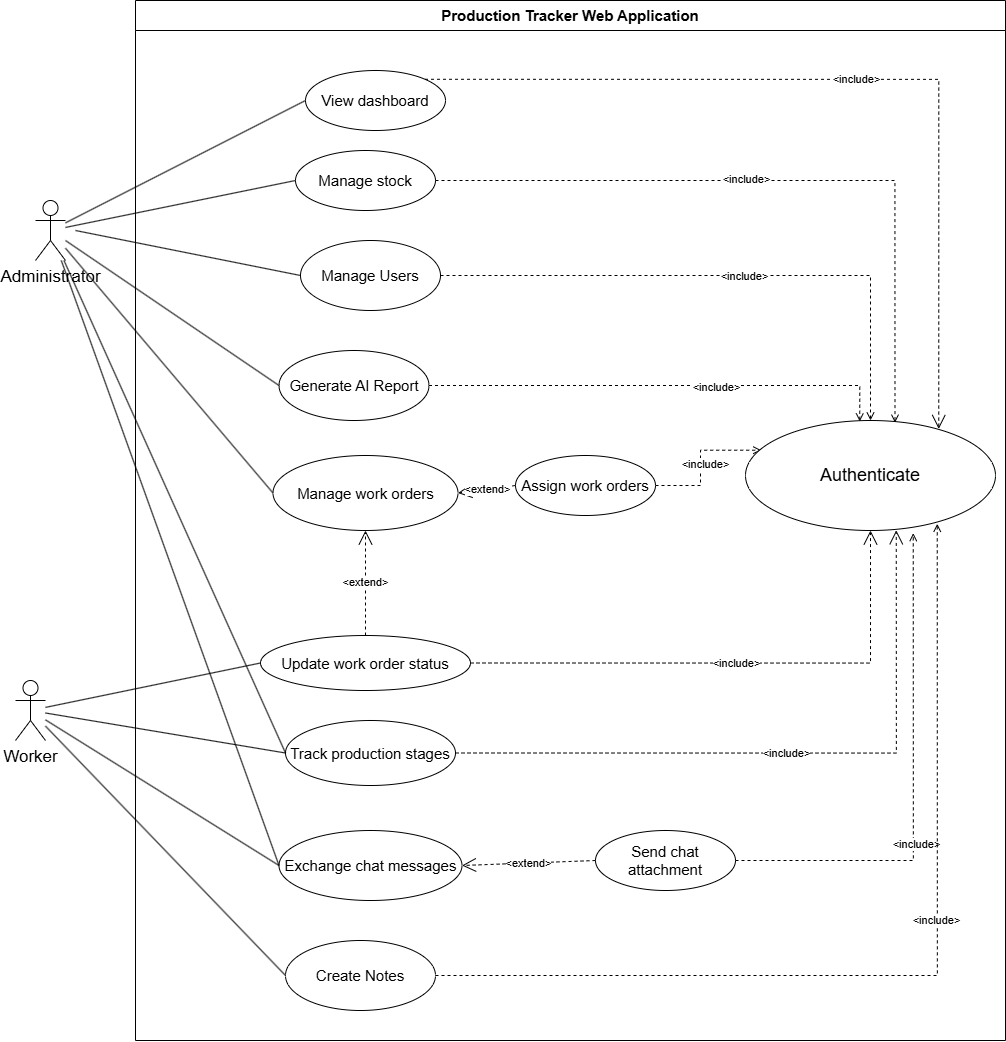
\includegraphics[width=\textwidth,keepaspectratio]{pictures/use caseFinal.drawio.png}
    \vspace*{\fill}
    \caption{Use Case Diagram}
    \label{fig:chapter2-use-case-diagram}
\end{figure}
\section{Global class diagramm}
the figure \ref{fig:chapter2-class-diagram} illustrates the global class diagram of the system.
\begin{sidewaysfigure}
    \centering
    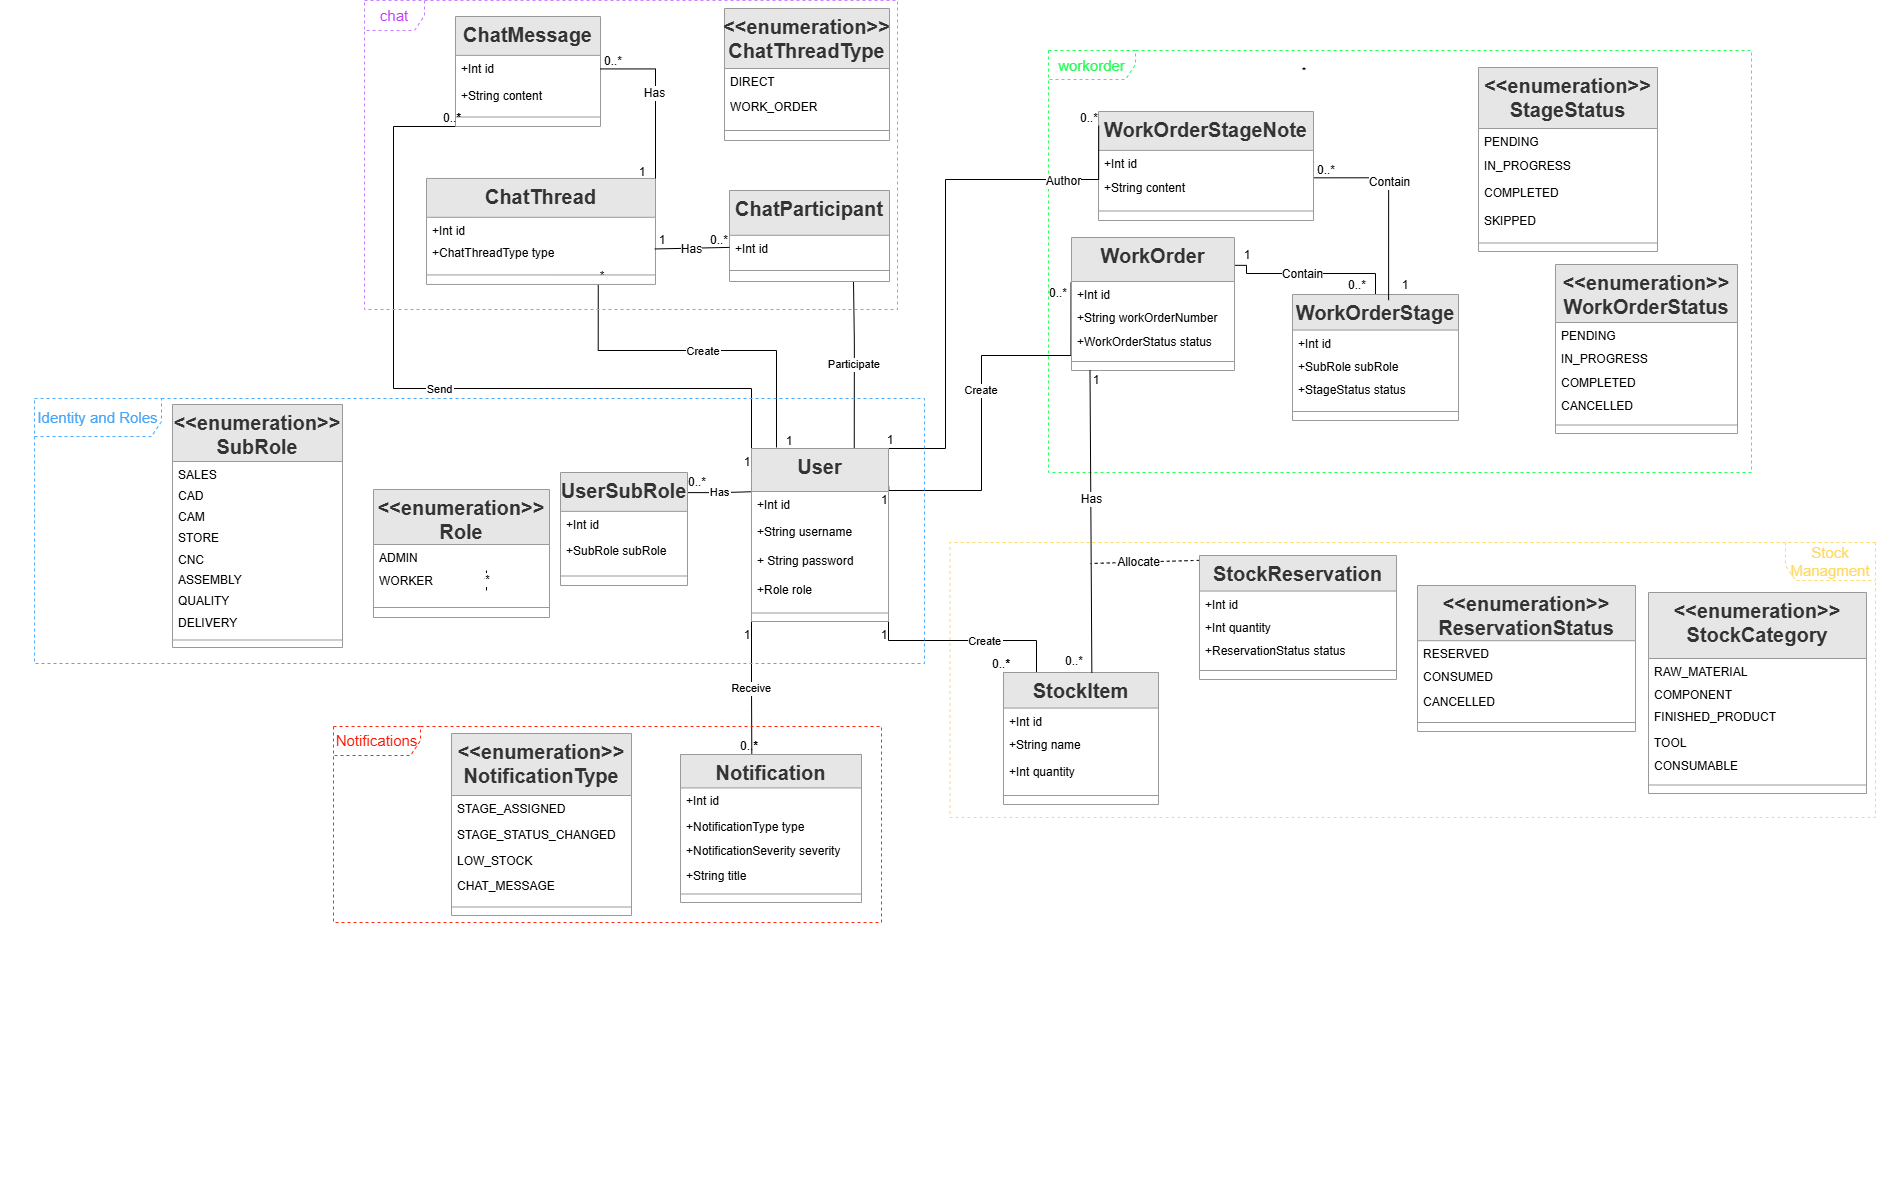
\includegraphics[width=0.95\textheight]{pictures/Class Diagram2.drawio.png}
    \caption{Global class diagram}
    \label{fig:chapter2-class-diagram}
\end{sidewaysfigure}
\section{Planning}
\subsection{Product backlog}
in this section we present the product backlog, which is a prioritized list of features and requirements that will guide the development process. Each item in the backlog is defined as a user story, which describes a specific functionality from the perspective of the end user. The backlog is organized into sprints, with each sprint focusing on a set of related features that will be developed and delivered together. The Table \ref{tab:product-backlog} represents the global Product backlog.
\footnotesize
\begin{longtable}{|p{0.08\textwidth}|p{0.24\textwidth}|p{0.48\textwidth}|p{0.14\textwidth}|}
    \caption{Product backlog}\label{tab:product-backlog}\\
    \hline
    \textbf{ID} & \textbf{Fonctionality} & \textbf{User Story} & \textbf{Actor} \\
    \hline
    \endfirsthead

    \hline
    \textbf{ID} & \textbf{Fonctionality} & \textbf{User Story} & \textbf{Actor} \\
    \hline
    \endhead

    \hline
    \endfoot

    \hline
    \multicolumn{4}{|l|}{\textbf{Sprint 1: Foundation and Access Control}} \\
    \hline
    PB-01 & User Authentication & As an administrator, I want to log in securely so that I can access protected management features. & Administrator \\
    \hline
    PB-02 & Role-Based Access Control & As an administrator, I want role-based permissions so that users only access features related to their role. & Administrator \\
    \hline
    PB-03 & User Management & As an administrator, I want to create, update, and deactivate user accounts so that I can manage the team effectively. & Administrator \\
    \hline
    PB-04 & Session Security & As a user, I want secure session handling with token expiration so that my account remains protected. & Administrator / Worker \\
    \hline
    \multicolumn{4}{|l|}{\textbf{Sprint 2: Work Orders and Stage Tracking}} \\
    \hline
    PB-05 & Work Order Creation & As an administrator, I want to create work orders with required details so that production tasks are clearly defined. & Administrator \\
    \hline
    PB-06 & Work Order Assignment & As an administrator, I want to assign work orders to workers so that each task has a responsible person. & Administrator \\
    \hline
    PB-07 & Work Order Status Tracking & As a worker, I want to update the status of my assigned work orders so that progress is visible to the administrator in real time. & Worker \\
    \hline
    \multicolumn{4}{|l|}{\textbf{Sprint 3: Stock Management}} \\
    \hline
    PB-08 & Inventory Registration & As an administrator, I want to register stock items with unique identifiers so that materials can be tracked accurately. & Administrator \\
    \hline
    PB-09 & Stock Reservation & As a worker, I want to reserve stock items for my tasks and mark them as consumed when used. & Worker \\
    \hline
    PB-10 & Reservation Tracking & As an administrator, I want to monitor stock reservations so that inventory usage is auditable. & Administrator \\
    \hline
    \multicolumn{4}{|l|}{\textbf{Sprint 4: Notes and Notifications (Real-Time Chat included)}} \\
    \hline
    PB-11 & Stage Notes & As a worker, I want to add notes on work stages so that operational details are documented for traceability. & Worker \\
    \hline
    PB-12 & Notification Center & As a user, I want to receive notifications for assignments, updates, and messages so that I do not miss important events. & Administrator / Worker \\
    \hline
    PB-13 & Real-Time Chat & As a user, I want to chat with other users in real time so that I can discuss issues and coordinate. & Worker / Administrator \\
    \hline
    PB-14 & File Sharing in Chat & As a user, I want to attach files in chat so that I can share production documents and evidence. & Administrator / Worker \\
    \hline
    \multicolumn{4}{|l|}{\textbf{Sprint 5: QR Codes, Analytics, and AI Reporting}} \\
    \hline
    PB-15 & QR Code Generation & As an administrator, I want generated QR codes for work orders so that identification is faster. & Administrator \\
    \hline
    PB-16 & QR Code Scanning & As a user, I want to scan QR codes so that I can quickly search and access work orders. & Worker / Administrator \\
    \hline
    PB-17 & AI Reporting Engine & As an administrator, I want AI-assisted reporting so that I can make faster data-driven decisions. & Administrator \\
    \hline
    PB-18 & Analytics Dashboard & As an administrator, I want an analytical dashboard for production data so that I can monitor KPIs and trends. & Administrator \\
    \hline
\end{longtable}
\normalsize
\subsection{Sprint Planning}

The internship lasted three and a half months, so the sprint planning was distributed accordingly.

The table \ref{tab:sprint-plan} summarizes the sprint plan by priority and period.

\begin{table}[H]
    \centering
    \caption{Sprint Plan} \label{tab:sprint-plan}
    \label{tab:sprint-planning}
    \begin{tabular}{|p{2.8cm}|p{4.6cm}|p{2.2cm}|p{2.6cm}|}
        \hline
         & \textbf{Sprint} & \textbf{Priority} & \textbf{Period} \\
        \hline
        \multirow{3}{*}{Release 1} & Foundation and Access Control & 1 & 21 days \\
        \cline{2-4}
         & Work Orders and Stage Tracking & 2 & 21 days \\
        \cline{2-4}
         & Stock Management & 3 & 21 days \\
        \hline
        \multirow{2}{*}{Release 2} & Notes and Notifications & 4 & 21 days \\
        \cline{2-4}
         & Real-Time Chat, QR Codes, AI Reporting & 5 & 21 days \\
        \hline
    \end{tabular}
\end{table}


\section{Conclusion}
\label{sec:conclusion-analysis}
This chapter provided a detailed analysis and specification of the requirements for the production tracking platform.Throughout this chapter, We identified the main actors involved in the system, 
defined functional and non-functional specifications to make sure the platform meets the company's needs,
outlined the technical environment,
In addition, we created several UML diagrams, including use case and class diagrams to provide a clear understanding of the system's behavior.
Finally The detailed product backlog will serve as a roadmap for the development process and will guide the implementation of the platform.
in the next chapter, we will start the implementation of the first release, which focuses on the development of the first three sprints.    